% -----------------------------------------------------------------------------
\section{Purpose}
% -----------------------------------------------------------------------------
% Synthetic biology aims to apply engineering principles such as standardization, modularity, and design abstraction to molecular biology.  However, synthetic biology still faces substantial challenges, including long development times, high rates of failure, and poor reproducibility. 

% The Synthetic Biology Open Language is intended to help synthetic biologists collaborate by allowing them to exchange designs in a standardized data format.  In addition, the SBOL data model systematically describes the essential details of a design that are required for researchers to reproduce each other's designs in the laboratory.  The purpose of the Synthetic Biology Open Language is to aid collaboration between researchers, improve scientific reproducibility, and to speed the research and development of technologies based on synthetic biology.

% Below is my revision. Any thoughts? - Nic
\Ctodo{Goksel:I find this paragraph too detailed. Up to the sentence starting with "When designing" is ok. If we really want to give an example, just a TF would be enough without mentioning about microRNAs or antagonists, and keeping it short.}
Synthetic biology builds upon the techniques and successes of genetics, molecular biology, and metabolic engineering by applying engineering principles to the design of biological systems. These principles include standardization, modularity, and design abstraction. The field still faces substantial challenges, including long development times, high rates of failure, and poor reproducibility. A common factor of these challenges is the exchange of information about designed systems between laboratories. When designing a synthetic system,  synthetic biologists need to exchange information about multiple types of molecules and their planned roles in the design. Often the functional role may be associated with another type of molecule entirely, such as a small chemical, a DNA, an RNA or a Protein molecule. An example is a DNA sequence that is transcribed into a messenger RNA that contains an encoded microRNA binding site, and the messenger RNA in turn being translated into a protein molecule which is a transcription factor binding protein. Functionally the representation of the products of the designed DNA sequence need to describe the role of microRNA binding to the messenger RNA leading to possible  degradation, the functional consequence of the transcription factor protein being absent leading to repression of expression of another gene and the kinetic information associated with these different elements so they can be mathematically modeled. The DNA sequence itself is thus one or two steps removed from the functional role of the designed device or circuit.


The \emph{Synthetic Biology Open Language} has been designed as a standard to support synthetic biology, filling a need not satisfied by other pre-existing standards. Previous file formats such as GenBank and Swiss-Prot represent sequence information based upon annotation of sequence features - they do not represent the functional roles or consequences of these sequences. Modelling languages, such as the Systems Biology Markup Language (SBML) ~\cite{SBML} can be used represent biological processes, but is not sufficient to represent the associated nucleotide or amino acid sequences.  %Goksel: Commented this sentence: Kinetic information may be present in SBML~\cite{SBML} or mass conservation laws in other systems such as the COBRA Toolbox~\cite{COBRA}. 
Synthetic biology needs a structured standard with defined ways on how to represent relevant molecules and their functional roles within the designed system, standardized rules on how such information is encoded in the file and the means to enable exchange of such data between participating laboratories as part of publications. 
%Goksel: Updated the sentence as above:Systems Biology Markup Language (SBML) represents reactions, pathways, and models, but does not typically represent the associated sequences.

To help address these challenges, the SBOL introduces a standardized format for the electronic exchange of information describing the structural and functional aspects of biological designs. 
The standard is designed to support the development of explicit and unambiguous data models of biological designs through the use of a well defined data model on how to represent the biological molecules, and their structural and functional roles in a systematic fashion. 
The standard further describes rules and best practices on how to include, develop, and populate this format with relevant information of essential design details. 
SBOL uses existing Semantic Web resources such as biological ontologies and \emph{Universal Resource Identifiers} (URIs) to unambiguously define genetic design elements.
%Goksel: Replaced thi sentence with the one above:Because the standard itself can represent information from other sources for sequence representations, reaction information and ontologies to represent biological design information, the standard uses modern information exchange techniques such as \emph{Universal Resource Identifiers} (URIs). This permits the reuse of existing information without the need to repeat it, thus avoiding both redundancy and likely future information decay within shared files. 
%Goksel: Removed this sentence: The ultimate utility of URIs in the SBOL standard is the ability to support flexible annotation with appropriate metadata while associating an authority with that annotation. 
The definition of the data model and associated format, the rules on the addition of data within the format and the representation of this in electronic data files are intended to make the SBOL standard a useful means of promoting global data exchange between laboratories and between software programs.

This document presents the second version of SBOL.
The previous version 1.1 of the SBOL standard focused on representing the structural aspects of genetic designs. 
Users of the standard were able to use it to exchange information on DNA designs but could not represent molecules other than DNA or represent the functional aspects of their designs beyond the DNA sequences. 
To serve as an effective medium for the computational exchange of genetic designs, SBOL must be extended to capture more aspects of a designed system, including both structural and functional information, and the composition of complex structural and functional designs by combining simpler parts. 
The SBOL 2.0 data model defined in this specification thus extends the prior model to provide for addressing the most pressing needs for expanding SBOL version 1.1, in particular it can:
\begin{itemize}

\item represent structural components of a biological design, including DNA, RNA, proteins, small molecules and other physical components

\item describe behavioral aspects of a biological design, the intended or expected interactions and dynamic behavior

\item associate structure and function together, so that a single design can be understood both in terms of its structure and its behavior

\item support rich annotations of all components, so that data required to describe a design, but not formalized in this specification can be safely exchanged

\end{itemize}
Taken together, these capabilities allow SBOL sufficient expressiveness to support the description and exchange of hierarchical, modular representations of both the intended structure and function of designed biological systems.

\begin{figure}
\centering
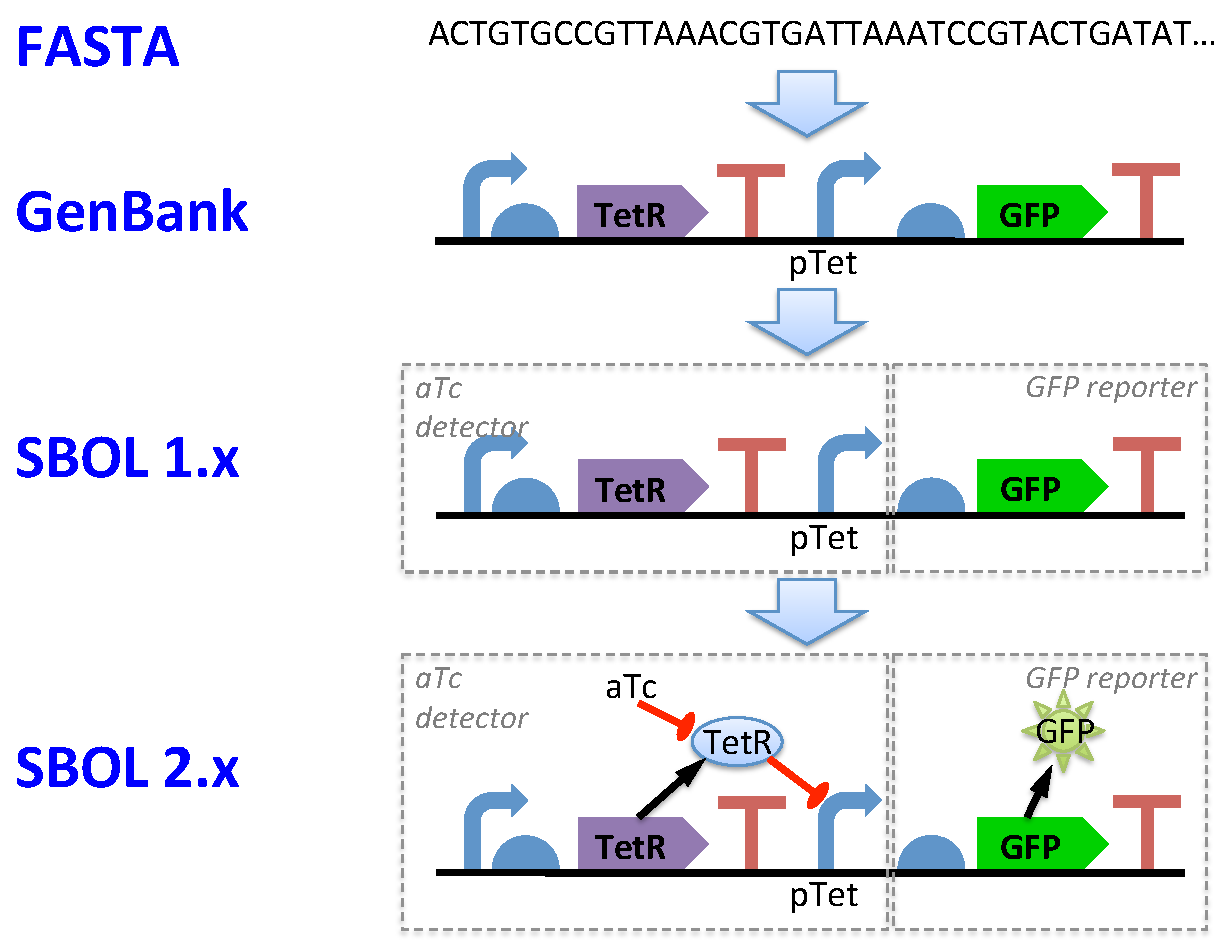
\includegraphics[width=5in]{images/format-comparison.pdf}
\caption{SBOL 2.0 extends prior formats to represent both structure and function of a genetic design in a single model.}
\end{figure}

\Ctodo{Figure is not referenced in the text and moved to where it is referenced. -CJM. Goksel: We need to redraw the figure with SBOL-Visual icons.}

To address the need for functional descriptions in SBOL, the proposed data model adds new classes to provide a firm basis for functional representation in SBOL without going so far as to create a new standard for mathematically modeling biology, as there already exist several established languages for doing so, from the SBML to CellML~\cite{CellML} and even MatLab~\cite{matlab}. Rather, these classes enable users of SBOL to group components that function together, describe the basic qualitative interactions between these components, and document references to standard mathematical models that are external to SBOL and that provide more detailed descriptions of component function. In other words, a module definition gathers together a set of component instantiations, a set of interactions between these component instantiations, and a set of references to external models that are expected to be consistent with the module's interactions.

The SBOL 2.0 specification also adds a number of measures to simplify adoption and validation of compatibility with the standard.
First, the specification explicitly incorporates its serialization format into the specification, whereas SBOL 1.1 used an implicit standard tied to a reference implementation.
Second, the specification includes a set of validation rules for determining compatibility of a document with SBOL 2.0, most of which are machine-verifiable.
Finally, the specification includes a set of recommended best-practices likely to allow a tool to take best advantage of the standard and other compatible tools.

Care has been taken to ensure that SBOL 2.0 is backward-compatible with SBOL 1.x.  
The generalization of the data model does mean that many names have changed and thus an SBOL 1.x file is not a valid SBOL 2.0 file.
There is, however, a direct mapping from the SBOL 1.x data model into the SBOL 2.0 data model, making it simple to automatically ``upgrade'' any SBOL 1.x file into and SBOL 2.0 file.
% Goksel - Removed this sentence:Therefore, SBOL 2.0 supersedes SBOL 1.1, and developers are encouraged to use it for all new software efforts.  
Since SBOL 2.0 can encode all data previously encoded in SBOL 1.1, developers are also encouraged to upgrade their SBOL 1.1 compliant software tools to use SBOL 2.0 data objects. 

\Rtodo{Added text above to address Swapnil's comment.  Needs review.  -CJM. Goksel: Went through this and removed the previous sentence to remove duplication.}

\Rtodo{I added this to bring extensibility to the fore as I thikn it is a crtical component of SBOL 2.0. Currently it is discused too late into the document and in a technical way that may not understandable by non-technical readers. The text will probably require some additional editing - HMS.}

As discussed previously, SBOL 2.0 allows designs to be described beyond the simple annotated DNA sequence offered in SBOL 1.1. Of equal importance in SBOL 2.0 is the explicit provision of mechanisms that allows SBOL to be easily extended~\cite{sec:Annotations}. The intent of SBOL is to allow designs of synthetic biological systems to be fully described so that such designs can be reproduced. However SBOL does not currently offer a full catalog of data%Note I'm using data not metadata to avoid technical terms at this state
to allow one to achieve complete reproducibility. For example the proposed standard does not yet include environmental and host context information or details on how the performance of the design is measured. Such details can now be included in SBOL through an explicit extension mechanism. Three scenarios are envisaged for extending SBOL:

\Rtodo{One might feel that the following list probably should go to the end of the overview but I wanted somewhere to describe the use cases of extensions in plain language without introducing any comp sci technical terms, and the overview is already fairly technical. If people don't like these types of low level descriptions in the spec document which would be a reasonable concern, then I can suggest a second document that gives a non-technical description of SBOL 2.0 - HMS.}

\begin{itemize}
\item Use of the extension mechanism to include critical information related to the reproducibility of designs. For example, what growth media was used, what temperature were the organisms grown at, when were they harvested, was the DNA integrated into the host genome (if so here), or in a plasmid (what plasmid).
\item For tool makers, the extension mechanism allows tool specific information to be added to SBOL. Such information could include tool settings specific to the design that is being loaded, for example what windows should be opene or settings initialized. Tool makers could also include encrypted proprietary information related to the company or client in an extension. 
\item Non-essential information to reproducibility but nevertheless useful information for many users. There are many cases where a community of users require specific information not available in core of SBOL. Examples include visualization information, how the DNA was assembled, information on evolutionary stability, or specialist modeling information.
\end{itemize}

The extension mechanism is therefore a critical part of SBOL 2.0 and will allow others in the community to incoroporate either their own requirements for data into SBOL or contribute to community efforts to expand the scope of SBOL.


The SBOL standard has been developed in collaboration between both ``wet'' bench scientists and ``dry'' scientific modelers and tool designers active within the synthetic biology community. 
As with the earlier SBOL 1.1 standard, this community (open for any practitioner to join) has met to discuss, argue and agree upon needs that the SBOL standard should address. 
This information has then been used by developers within our community to design, develop, and test a specification of the standard. The specification has been tested by the community through several iterations for the ability to represent a wide range of synthetic biology design projects, as well as, the ability to share designs between different laboratories. 
The standard has also been used to develop software tools that employ the standard for developing and sharing synthetic design projects. 
The publication of this specification is intended to make these capabilities more widely accessible to the community of potential developers and users.